\chapter{Implementacja projektu}
\section{Moduł Arduino}
W tym projekcie wykorzystany został moduł Arduino w wersji Leonardo oparty na mikrokontrolerze AVR Atmega32U4. Posiada on 20 cyfrowych pinów wejścia/wyjścia z czego 12 z nich można ustawić jako analogowe. Co ważne dla tego projektu posiada on aż 5 pinów, które obsługują przerwania (więcej informacji w rozdziale 4.).
\subsection{Napięcia i zasilanie}
\subsubsection{Napięcia}
Moduł ten operuje na napięciu 5V, tak więc na każdym z portów wejścia/wyjścia nie może pojawić się większe napięcie, ponieważ grozi to zepsuciem układu. W przypadku samochodu, którego głównym napięciem jest napięcie z akumulatora \textasciitilde12V, trzeba zastosować elementy elektroniczne dostosowujące oba napięcia do siebie.
\subsubsection{Zasilanie}
Rekomendowane wartości napięcia, aby zasilić sam moduł według specyfikacji producenta musi zawierać się w przedziale 7-12V. Aby spełnić te warunki układ zasilania został skonstruowany na bazie stabilizatora 9V 7809 oraz kondensatorów. Moduł nie został podłączony bezpośrednio do obwodu w samochodzie, ponieważ podczas pracy alternatora napięcie w układzie jest większe niż maksymalne wymagane przez Arduino (dochodzi do \textasciitilde14V).

\begin{figure}[ht]
\centering
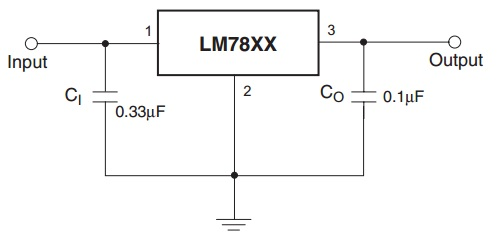
\includegraphics[width=0.7\linewidth]{Rysunki/78xx.jpg}
\caption{Schemat podłączenia układu zasilania \cite{LM78XX}}
\label{fig:LM78XX}
\end{figure}

\section{Podłączenie do pojazdu}
\subsection{Komputer pokładowy}
Aby możliwy był odczyt wymaganych parametrów do poprawnego działania projektu, potrzebna jest wiedza na temat schematu podłączeń komputera pokładowego (ECU) umieszczonego w samochodzie. Jak się okazało, ze schematu portów wejścia/wyjścia\cite{HondaPinout}, wszystkie potrzebne sygnały są wpięte do ECU. Sygnały te zostały opisane w tabeli~\ref{tab:ecu_pinout}

\begin{table}[htb] \small
\centering
\caption{Potrzebne wyprowadzenia według schematu ECU\cite{HondaPinout}}
\label{tab:ecu_pinout}
\begin{tabularx}{\linewidth}{|c|p{7cm}|c|c|X|} \hline\
\textbf{Oznaczenie} & \textbf{Opis} & \textbf{Wtyczka} &\textbf{ Pin} & \textbf{Kolor} \\ 
\hline
INJ1 & Przewód do wtrysku pierwszego & A & 1 & brązowy\\
\hline
VSS & Przewód czujnika prędkości & B & 10 & żółty\\
\hline
TPS & Przewód czujnika położenia pedału gazu & D & 11 & jasny zielony\\
\hline
\end{tabularx}
\end{table}

Aby podpiąć się do wyżej wymienionych przewodów zostały użyte bezinwazyjne szybkozłączki. 

\subsection{Czujnik prędkości}
Po pomiarach multimetrem okazało się, że impulsy w VSS mają dokładnie 5V, co oznacza, że nie potrzeba zastosowywać żadnych elementów elektronicznych, aby podłączyć się do modułu. Połączenie zostało więc stworzone bezpośrednio do pinu nr 7 obsługującego przerwanie nr 4.

\subsection{Sygnał wtrysku}
Pomiary wykazały, iż wtryski pracują na napięciu 12V, tak więc w tej sytuacji trzeba zastosowa element zmniejszający napięcie. Wybór padł na stabilizator 7805. Dodatkowe kondensatory nie zostały użyte jak w przypadku układu zasilania Arduino, ponieważ mogłyby one wpływać na dokładność pomiarów. Przewód ze zmniejszonym już napięciem został podpięty do pinu nr 2 obsługującego przerwanie nr 1.

\subsection{Czujnik położenia pedału gazu}
W tym wypadku, pomiary wykazały, że czujnik ten działa niczym potencjometr i zmienia napięcie od \textasciitilde0.5V dla pedału nie wciśniętego wcale, do \textasciitilde4.5V gdy pedał jest wciśnięty w 100\%. Wyprowadzenie te zostało podłączone do analogowego pinu A0.

\subsection{Podłączenie woltomierza}

Aby wyświetlić aktualne napięcie w układzie samochodu nie uszkadzając przy tym modułu (w układzie pojazdu panuje napięcie przewyższające 5V), zostanie użyty prosty obwód z dwoma rezystorami.

% schemat dodać

W ten sposób można modułem 5V mierzyć napięcie w zakresie 0-20V. Więcej informacji w kolejnym rozdziale.

\section{Podłączenie akcesoriów}

\subsection{Wyświetlacz LCD}
Wyświetlacz jaki został wybrany do projektu to znany model LCD ze 2x16 znaków o symbolu JHD162A-B-W zgodny ze sterownikiem HD44780. Został on połączony z Arduino poprzez cyfrowe piny: 12, 11, 6, 5, 4, 3. Dodatkowo został dołączony potencjometr do regulacji kontrastu wyświetlacza oraz zostało użyte dodatkowe połączenie służące do sterowania podświetleniem wyświetlacza - pin 9.

% schemat

\subsection{Mikro przełącznik}
Aby umożliwić użytkownikowi końcowemu sterowanie trybami pracy modułu został podłączony również mikro przełącznik. Został on przyłączony do pinu 13.

\subsection{Czujnik temperatury}
Dodatkową funkcją modułu będzie wyświetlanie aktualnej zewnętrznej temperatury. W tym celu został użyty cyfrowy czujnik temperatury DS18B20 w wersji wodoodpornej, 3 metrowej sondy. Czujnik ten umożliwia komunikację po interfejsie 1-Wire, dzięki któremu wystarczy tylko jedna linia, aby komunikować się z czujnikiem (więcej informacji w kolejnym rozdziale).

